En este capítulo se detalla el diseño del proyecto, basado en el análisis
mostrado en anteriormente. Entre otros detalles, se presenta la arquitectura
general y el diseño físico de datos.

\section{Arquitectura del sistema}

\subsection{Arquitectura física}
\label{sec:arquitectura-fisica}

En este apartado, describimos los principales componentes hardware que forman
la arquitectura física de nuestro sistema, recogiendo por un lado los componentes
del servidor de producción y, por otro lado, los componentes del cliente de acceso.

\subsubsection{Servidor de producción}
\label{subsec:entorno-produccion}

\paragraph{Hardware}

El \textit{hardware} mínimo indispensable para la correcta ejecución de la API
es el siguiente:

\begin{itemize}
\item 512MiB de memoria RAM.
\item 10GiB de disco duro.
\item Acceso a Internet con un canal de subida de al menos 1Mbit/s.
\end{itemize}


\paragraph{Software}

En cuanto al \textit{software} necesario para la ejecución del proyecto, se
detallan los siguientes elementos, que es necesario instalar para desplegar el
sistema:

\begin{itemize}
\item Sistema operativo \textbf{GNU/Linux}. Durante el desarrollo del proyecto y
  en el actual servidor de producción se utilizó Ubuntu.
\item Código fuente del proyecto \textbf{Amuse Bouche}.
\item Servidor de shell remota \textbf{SSH}, accesible desde el exterior.
\item \textbf{Nginx} como servidor web.
\item \textbf{Supervisord} como sistema para el control de procesos que trabajen
  en modo demonio.
\item \textbf{Python}, versión mínima 3.0.
\item Soporte de entornos virtuales \textbf{VirtualEnv} para la encapsulación de
  dependencias.
\end{itemize}

\subsubsection{Cliente de la aplicación Android}

Los usuarios que deseen utilizar la app deberán contar con un dispositivo que
soporte como mínimo la versión 4.0 del sistema operativo Android. Para la
instalación inicial se necesitará que posean acceso a internet y a los servicios
de Google Play. Posteriormente podrán utilizar la app sin conectarse, si así lo
desean.


\subsection{Arquitectura lógica}

La arquitectura lógica del sistema está formada por los elementos software
(servicios, aplicaciones, librerías, \textit{frameworks}, etc.) que componen el
software base, más el software desarrollado para cumplir los requisitos de la
aplicación. En esta sección se especficia la organización de los distintos
elementos software que componen el proyecto así como la comunicación entre
ellos. 

\subsubsection{Arquitectura de la API}
\label{subsec:arquitectura-logica-api}

En la figura~\ref{fig:arquitectura-logica-api} se puede ver un esquema de cómo se
comunican los diferentes elementos que conforma el sistema web a alto nivel. En
detalle, el flujo que sigue en cada capa es el siguiente.

\begin{figure}[htbp]
  \centering
  \includegraphics[width=0.9\textwidth]{cap5/img/diagrama_arquitectura_logica_api}
  \caption{Arquitectura lógica de la API}
  \label{fig:arquitectura-logica-api}
\end{figure}



\paragraph{Cliente}

Cuando usuario desea realizar una acción en la aplicación, esto se traduce como
enviar una petición \ac{HTTP} al servidor, es decir, se abre una conexión
\ac{TCP} al puerto 80 del servidor remoto y enviar las cabeceras en las cuales
debe indicarse qué datos se desean obtener o accción se desea llevar a cabo.

\paragraph{Servidor web}

Para que el servidor pueda escuchar dichas peticiones y responder a ellas, debe
tener en ejecución algún servicio que pueda hacerlo. Como ya hemos adelantado,
en el caso en que nos encontramos, se utiliza \textit{nginx}, un servidor web
que recibirá las peticiones HTTP hechas externamente.

Al tratarse de la obtención de una serie de recursos dinámicos (páginas generadas
dinámicamente, como es el caso) \textit{nginx} actuará como un proxy inverso y trasladará
la petición al manejador que corresponda.

\paragraph{Servidor de aplicaciones}

El manejador correspondiente en este proyecto es el servidor \textit{Gunicorn},
el cual está basado en el modelo \textit{pre-form worker}. Gunicorn instancia
varios procesos al lanzar el servidor que se encargarán de procesar las
peticiones de forma paralela, según el proceso padre las reparta.

En Python existe un estándar en el desarrollo web, conocido como \ac{WSGI}, una
especificación de una interfaz universal y simple entre los servidores web y
las aplicaciones web. Es decir, según este estándar se regula la forma en que
se comunica la aplicación con el servidor web. Entonces, cuando un proceso
recibe una petición se comunica con la interfaz WSGI de la aplicación que vaya
a ejecutar, traslandándole la petición y esperando que le informe cuando la
repsuesta esté lista.

\paragraph{Punto de entrada WSGI}

Como se ha comentado, el proceso del servidor de aplicaciones se comunica con la
interfaz WSGI. Todas las aplicaciones desarrolladas en Django cuentan con un
módulo \texttt{wsgi.py} que actúa como punto de entrada WSGI y que directamente
pasa la petición al \textit{middleware} del framework, que empieza el
procesamiento.

\paragraph{Framework web}

El framework escogido, como ya quedó especificado en la
sección~\ref{sec:alternativas-solucion}, es \textbf{Django}~\cite{django:mvc}. El
objetivo fundamental de este \textit{framework} es facilitar la creación de
sitios web complejos, haciendo especial hincapié en un ritmo de desarrollo
rápido y evitar la duplicidad de código. Por lo que el mayor potencial de Django
es la gran cantidad de funcionalidad que ya trae integrada, ya sea en el propio
núcleo del \textit{framework} o a través de módulos oficiales que se incluyen en
la distribución oficial.


\paragraph{Middleware Django y aplicación}

A partir de este punto, la petición va desplazándose entre código propio del
\textit{framework} Django y el código de la aplicación. El flujo habitual, en su
forma más básica es el siguiente:

\begin{enumerate}
\item Los módulos de \textit{middleware} que gestionan las peticiones reciben la
  petición actual.
\item Django revisa el fichero \texttt{urls.py} de la aplicación, que contiene
  una lista de URLs asociadas a funciones. Django compara la URL de la petición
  recibida y mira si coincide con alguna de las URLs del proyecto.
\item Si no hay coincidencia, Django devuelve una respuesta negativa,
  normalmente en forma de código de estado 404.
\item Si hay coincidencia, Django llama a la función asociada a esa URL, que
  procesa la petición, devolviendo una respuesta.
\item Esa respuesta hace el camino de forma inversa hasta volver al cliente.
\end{enumerate}

Cada aplicación en Django cuenta con una arquitectura de tres capas conocida
como \textbf{Modelo-Plantilla-Vista}, que es parejo al patrón del
\textbf{Modelo-Vista-Controlador}~\cite{django:mvc}.

\begin{itemize}
\item El \textbf{modelo} representa la información en la base de datos, evitando
  al usuario tener que utilizar código SQL. Para ello, Django cuenta con un
  \ac{ORM} que facilita el trabajo con registros de la base de datos.
\item Las \textbf{vistas} suelen ser funciones asociadas a una URL. La filosofía
  de Django es que las vistas sirvan solo como \textit{punto de paso} de los
  datos entre los modelos y las plantillas. Es mala práctica colocar lógica de
  negocio compleja en las vistas.
\item Las \textbf{plantillas} son la representación final de los datos, lo que
  acaba viendo el usuario. Las plantillas suelen estar escritas en HTML aunque
  pueden también representarse usando JSON, XML, etc.
\end{itemize}

La estructura de ficheros de un proyecto Django se ajusta, por tanto, a la
organización lógica hasta ahora descrita. Así, la raíz del proyecto contiene:
\begin{itemize}
\item \texttt{amuseapi} Directorio de proyecto a nivel global (para el caso en
  que existieran varias aplicaciones en un mismo proyecto)..
  \begin{itemize}
  \item \texttt{settings.py} Configuración general.
  \item \texttt{urls.py} Configuración de URLs.
  \item \texttt{wsgi.py} Punto de acceso WSGI.
  \end{itemize}
\item \texttt{recipes} Directorio de la aplicación de recetas.
  \begin{itemize}
  \item \texttt{models.py} Definición de modelos.
  \item \texttt{permissions.py} Definición de permisos.
  \item \texttt{serializers.py} Definición de serializadores (intermediarios
    entre las vistas y los modelos).
  \item \texttt{views.py} Definición de vistas (funciones).
  \item \texttt{tests.py} Definición de tests.
  \end{itemize}
\end{itemize}



\subsubsection{Aplicación Android}
\label{subsec:arquitectura-logica-android}

Android está construido con una arquitectura de 4 capas relacionadas entre
sí.~\cite{learning-android}. En la figura~\ref{fig:arquitectura-logica-app} se
puede ver que la estructura de Android se encuentra construida sobre el
\textit{kernel} de Linux. Luego hay una capa de bibliotecas relacionadas con una
estructura administradora en tiempo de ejecución. En el siguiente nivel
encontramos un \textit{framework} de apoyo para construcción de aplicaciones y,
por último, tenemos la capa de las aplicaciones.

\begin{figure}[htbp]
  \centering
  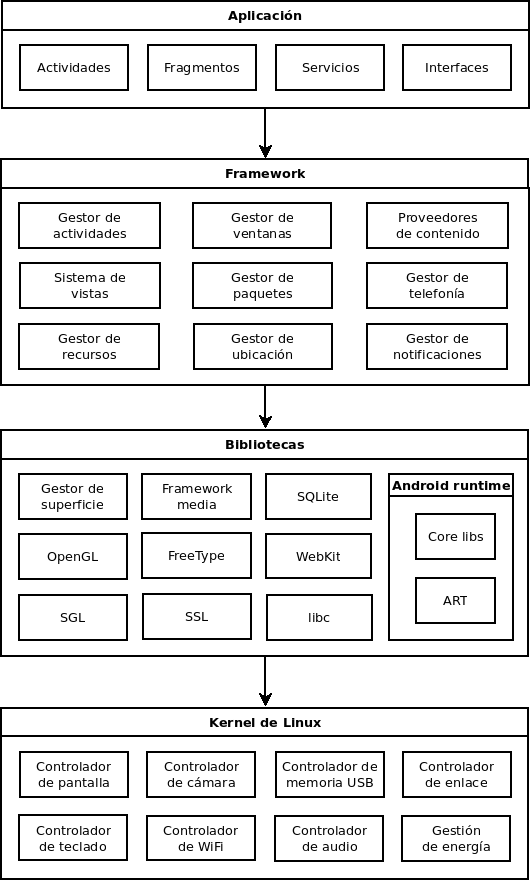
\includegraphics[width=0.9\textwidth]{cap5/img/diagrama_arquitectura_logica_app}
  \caption{Arquitectura lógica de la app}
  \label{fig:arquitectura-logica-app}
\end{figure}


\paragraph{Kernel de Linux}

Android está construido sobre el núcleo de Linux, modificado para adaptarse a
dispositivos móviles. Esta elección está basada en la excelente flexibilidad y
seguridad que Linux presenta. Ya que el \textit{kernel} de Linux se encuentra
licenciado bajo \ac{GPL}, Android también lo está.



\paragraph{Bibliotecas}

Entre las bibliotecas que forman parte de esta capa se encuentran las
siguientes:
\begin{description}
\item[Capa de abstracción del hardware] Permite la independencia del hardware,
  es decir, añade la capacidad de poder ejecutar el sistema en cualquier
  dispositivo móvil sin importar su arquitectura física. Este sistema actúa
  como una arquitectura genérica que representa todos los posibles tipos de
  hardware existentes en el mercado. Aunque por el momento no hay estándares de
  construcción en el hardware de dispositivos móviles, la capa de abstracción
  permite que cada fabricante ajuste sus preferencias para que Android pueda
  funcionar sobre ella.
  
\item[Bibliotecas nativas] Son las interfaces de código abierto para múltiples
  usos, como OpenGL para el renderizado de gráficos 3D, SQLite para la gestión
  de bases de datos, WebKit para el renderizado en navegadores, ... También
  existen bibliotecas para soportar los servicios del sistema como el Wifi,
  el GPS y la telefonía, entre otros.
  
\item[Demonios] Son programas que están en segundo plano ejecutándose, esperando
  algún tipo de llamada o evento para ser lanzados.

\item[Máquina virtual] Las aplicaciones Android están escritas en lenguaje Java
  y son traducidas a \textit{bytecode}, como las aplicaciones Java tradicionales.
  Sin embargo, éstas no son interpretadas por la máquina virtual de Java tal y
  como lo hacían las otras. Android tiene su propia máquina virtual.

  Era necesario construir una máquina virtual específica por varios motivos:
  el primero y más esencial es que la \ac{JVM} no tiene licencia GPL, y la
  segunda es que se necesitaba que fuera flexible ante el diseño de hardware de
  un dispositivo móvil. Así, Google creó su propia máquina virtual.

  Desde la versión 2.2 de Android, se utilizaba para este fin la máquina virtual
  Davil. Sin embargo, con la llegada de Android 4.4, ART debutó como entorno de
  ejecución alternativo y reemplazó completamente a Dalvik a partir de Android
  5.0 Lollipop. \ac{ART}~\cite{art-and-dalvik} es un entorno de ejecución de
  aplicaciones que lleva a cabo la transformación de la aplicación en
  instrucciones de máquina, que luego son ejecutadas por el entorno de ejecución
  nativo del dispositivo.  

  La construcción de una aplicación Java empieza por traducir el código fuente
  con el compilador de Java, javac, para obtener el código \textit{bytecode}
  contenido en archivos \textit{.class}. Al final, la JVM interpreta en tiempo
  real estos archivo y la aplicación es ejecutada.

  Cuando se usaba Dalvik, la construcción de una aplicación Android se basaba en
  que el compilador de Java tradujera la aplicación a \textit{bytecode}, y
  entonces el compilador Dex compilara este código a \textit{bytecode} nativo que
  será convertido en un ejecutable \textit{.dex}. Finalmente este archivo es
  ejecutado por una instancia de Dalvik VM.
  
  Para mantener la compatibilidad con versiones anteriores, ART utiliza el mismo
  \textit{bytecode} de entrada que Dalvik, el cual es suministrado a través de
  archivos \textit{.dex} estándar como parte de los archivos \ac{APK}, mientras
  que los archivos \textit{.odex} son reemplazados por archivos de formato
  ejecutable y enlazable (ELF). Una vez que una aplicación se compila utilizando
  ART en el dispositivo, ésta es dirigida exclusivamente a partir del ejecutable
  ELF compilado. Este enfoque elimina diversos gastos involucrados con la
  compilación JIT, pero requiere de tiempo adicional para la compilación cuando
  se instala la aplicación. También las aplicaciones ocupan cantidades
  ligeramente mayores de espacio de almacenamiento para almacenar el
  \textit{bytecode} compilado.

  Toda la arquitectura comentada está esquematizada en la
  figura~\ref{fig:arquitectura-art}.   

\begin{figure}[htbp]
  \centering
  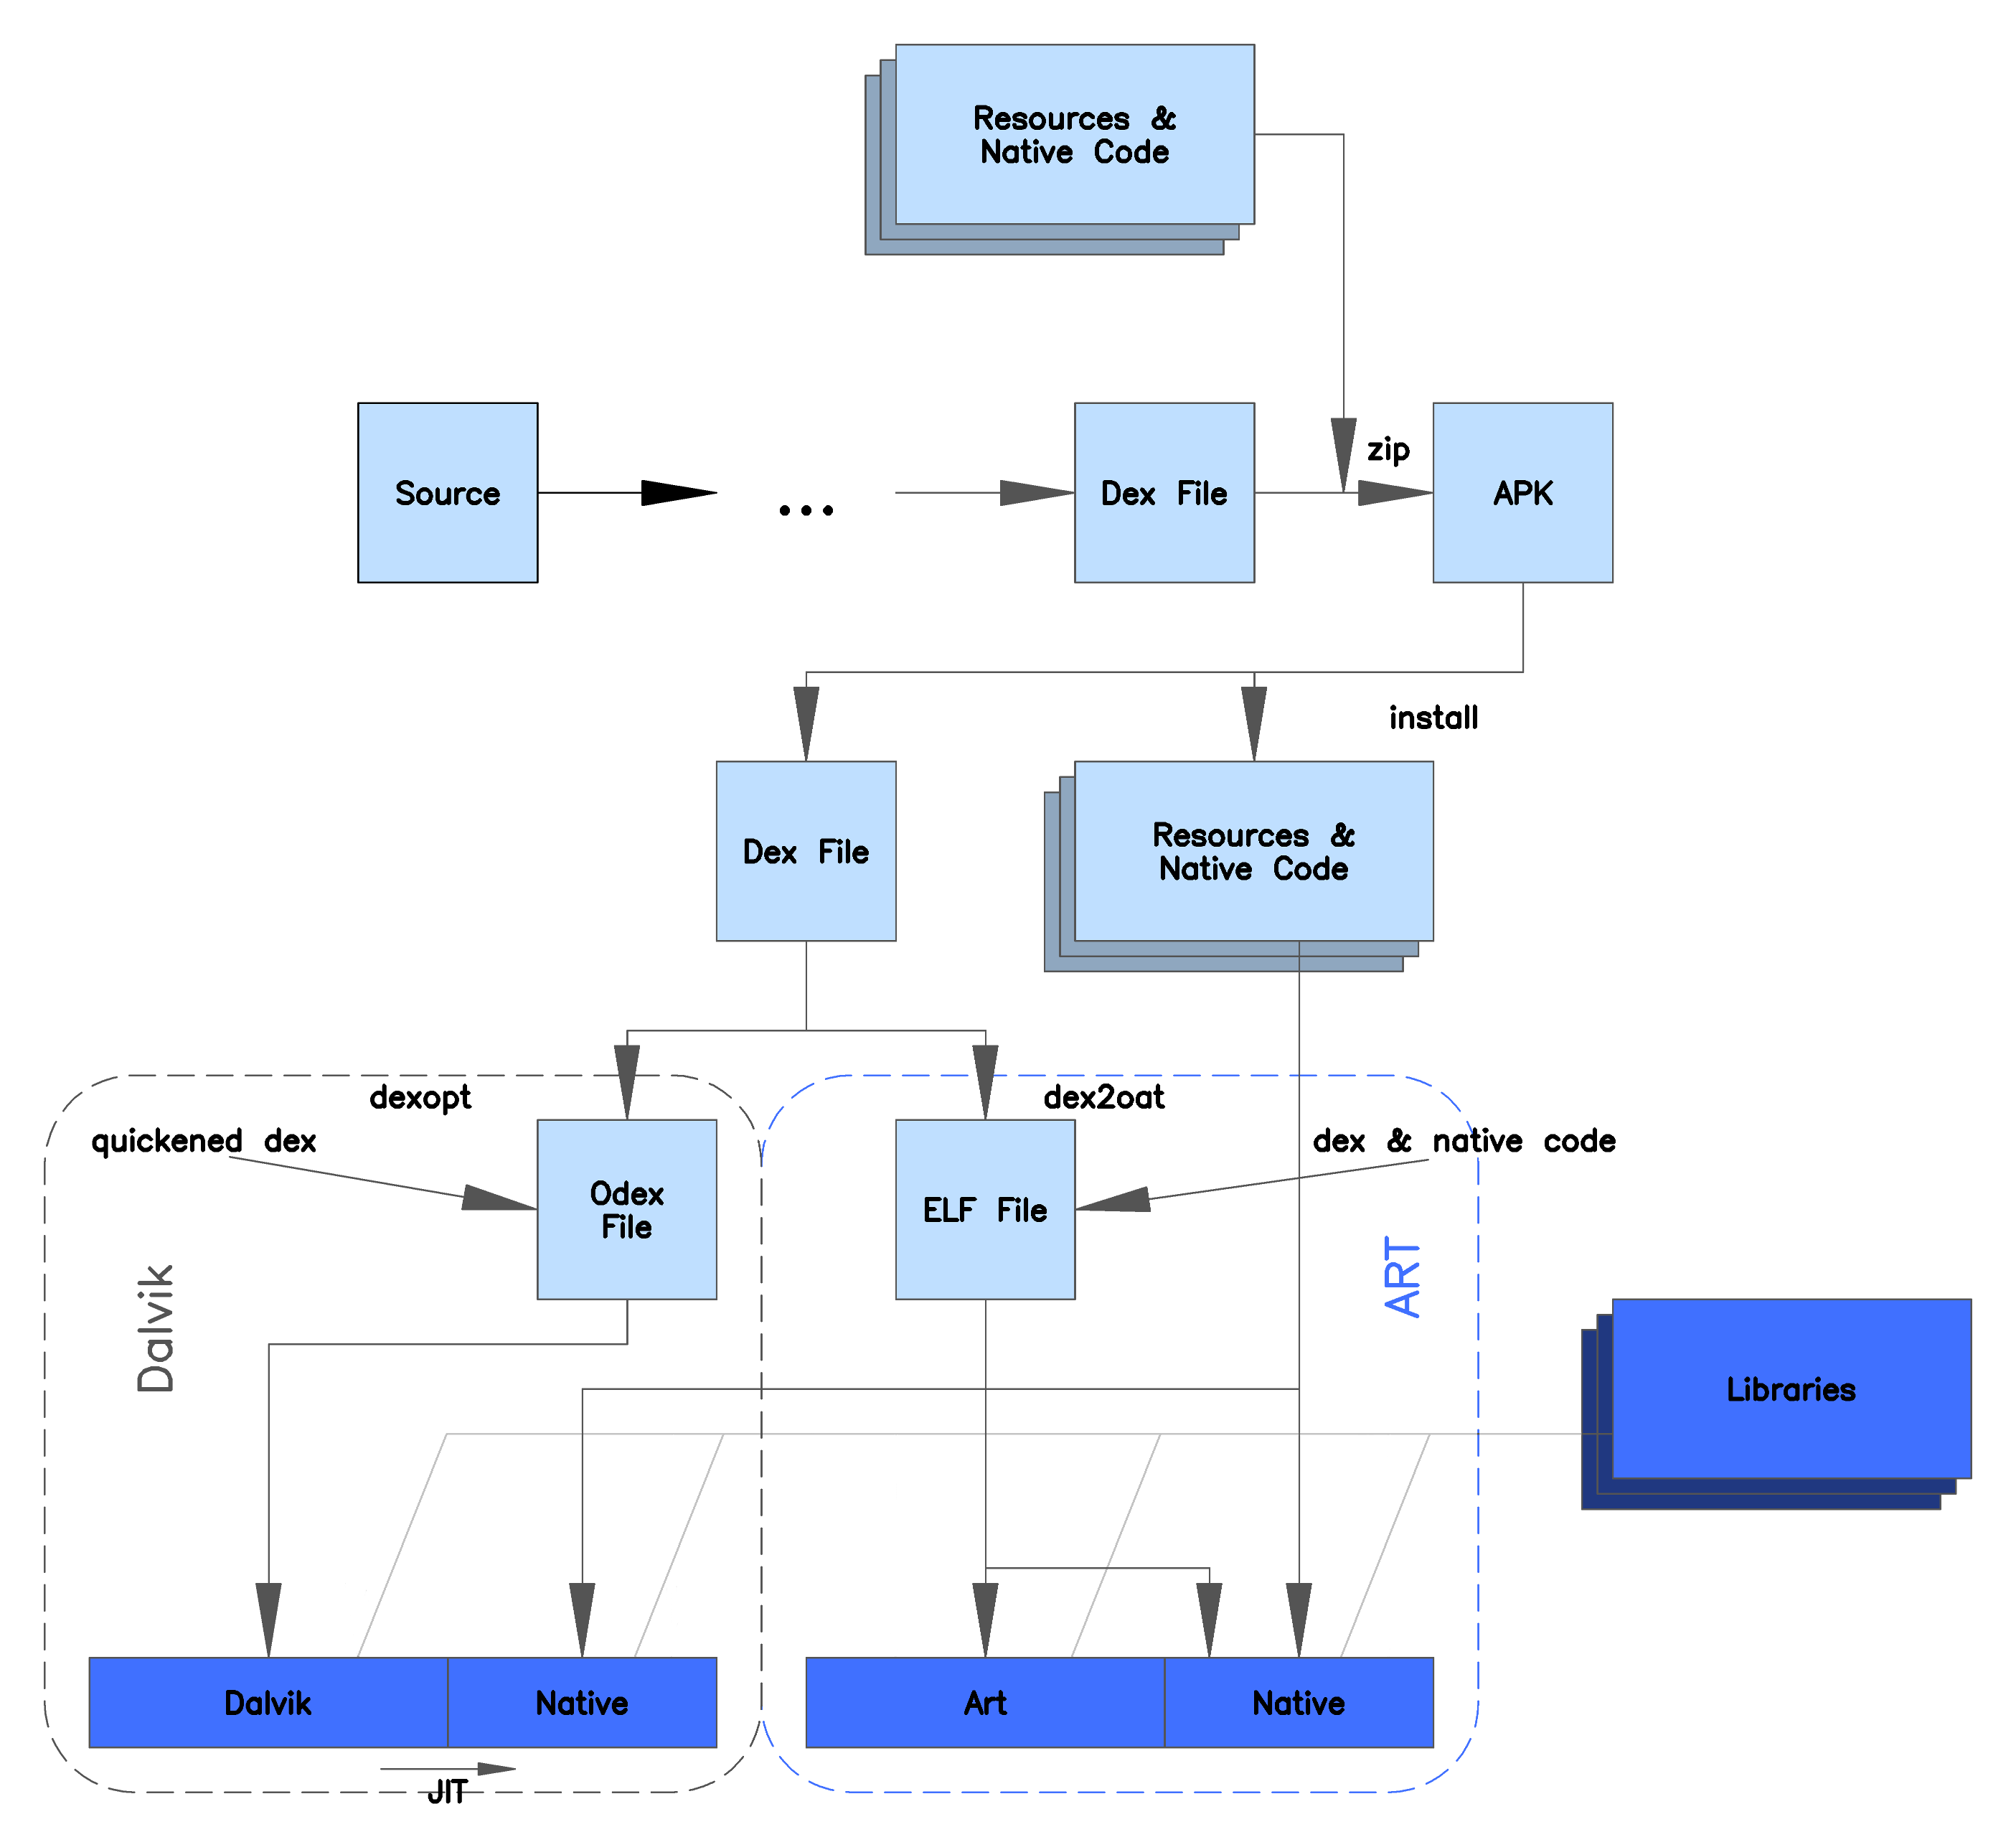
\includegraphics[width=0.9\textwidth]{cap5/img/ART}
  \caption{Diagrama de la arquitectura de Android Run Time}
  \label{fig:arquitectura-art}
\end{figure}
\end{description}


\paragraph{Framework para aplicaciones}

En esta capa todas las bibliotecas Java que se necesitan para programar las
aplicaciones. Los paquetes más utilizados son los empaquetados en
\texttt{android.*}, ya que en ellos se encuentran todas las características
necesarias para construir una aplicación Android, aunque también es posible
acceder a clases como \texttt{java.utils.*}, \texttt{java.net.*}, ... (salvo
aquellas bibliotecas excluidas, como \texttt{java.awt.*} y
\texttt{java.swing.*}).

En esta capa también encontraremos manejadores, servicios y proveedores de
contenido que soportan la comunicación de nuestra aplicación con el ecosistema
de Android.


\paragraph{Aplicaciones}

Es la última instancia de funcionamiento de Android. A este nivel acceden todos
los usuarios Android debido a su alto nivel de compresión y simplicidad.

El resultado del proceso de construcción de una app es un archivo comprimido con
formato APK (Android Applicacion Package\footnote{Un archivo APK es básicamente
  un archivo ZIP con una extensión diferente}), con la siguiente estructura:

\begin{itemize}
\item \texttt{META-INF}:
  \begin{itemize}
  \item \texttt{MANIFEST.MF}: El archivo Manifest.
  \item \texttt{CERT.RSA}: El certificado de la app.
  \item \texttt{CERT.SF}: La lista de recursos y recopilcación de SHA-1
    correspondientes al manifest.
  \end{itemize}
\item \texttt{lib}: Directorio que contiene el código compilado que es
  específico de una capa de software de un procesador.
  \begin{itemize}
  \item \texttt{armeabi}: Código compilador para procesadores basados en ARM
  \item \texttt{armeabi-v7a}: Código compilador para procesadores basados en
    ARMv7 o superior.
  \item \texttt{x86}: Código compilado para procesadores x86.
  \item \texttt{mips}: Código compilado para procesadores MIPS.
  \end{itemize}
\item \texttt{res}: Directorio que contiene los recursos no compilados en
  \texttt{resources.arsc}.
\item \texttt{assets}: Directorio que contiene los assets de la app, que pueden
  obtenerse mediante el \textit{AssetManager}.
\item \texttt{AndroidManifest.xml}: Un archivo manifest adicional, que describe
  el nombre, la versión, los derechos de acceso, archivos de biblioteca que se
  hace referencia para la aplicación.
\item \texttt{classes.dex}: Las clases compiladas en formato \textit{dex}.
\item \texttt{resources.ars}: Archivo que contiene recursos precompilados.
\end{itemize}

Este archivo APK se genera utilizando una herramienta de automatización: Gradle.
Se encarga de compilar, empaquetar, testear y liberar aplicaciones.


Una de las mayores ventajas de usar Gradle es que permite al desarrollador
modificar el flujo de construcción. Esto quiero decir que se puede decidir el
orden de ejecución de tareas. Asimismo podríamos elegir que archivos compilar
primero, cuando detener la compilación o establecer condiciones para que se
recompile o no el código.

Además Gradle permite ejecuciones incrementales, por lo que ahorra al
programador gran cantidad de tiempo de espera. También permite que construyamos
varias versiones de nuestra aplicación (para varias versiones de Android).

Otro detalle muy interesante es que se pueden ejecutar tareas en hilos
diferentes para optimizar el proceso de construcción.


\section{Diseño detallado de componentes}

TODO


\section{Diseño físico de datos}

TODO


\section{Diseño de la imagen corporativa}

La imagen corporativa del proyecto comprende el diseño del logotipo, la elección
de la paleta de colores y las tipografías, que se usan en el diseño de la app y
cualquier otro elemento visual.

El diseño completo se ha basado en
\textit{Material Design}.\cite{material-design} Este diseño recibe su nombre por
estar basado en objetos materiales: piezas colocadas en un espacio (lugar) y con
un tiempo (movimiento) determinado.

Es un diseño donde la profundidad, las superficies, los bordes, las sombras y
los colores juegan un papel principal.

Algunos detalles importantes a la hora de abordar el diseño son:
\begin{itemize}
\item Utilizar una tipografía clara, casillas bien ordenadas, colores e
  imágenes llamativos para no perder el foco y un sentido del orden y la
  jerarquía muy marcado.
\item También es necesario crear una iluminación realista que proporcione
  indicios de cómo se comportará un elemento y en qué nivel se encuentra.
\item Crear animaciones y movimientos, que indiquen el flujo a seguir.
\end{itemize}


\subsection{Nombre del proyecto}

El propio nombre del proyecto también forma parte de la imagen corporativa. Dada
la naturaleza del proyecto y lo que se buscaba conseguir, se trataba de buscar
un nombre atrayente relacionado con la comida, algo que llamara más la atención
que un simple \textit{``Tu recetario de cocina''}.

Investigando un poco, hay un concepto propio de la cocina
francesa,\cite{gastronomia-francia} denominado \textit{``amuse-bouche''}. No hay
nada más relacionado con la cocina que el francés, dado que la gastronomía
francesa es una de las más importantes del mundo, tanto culturalmente como por
sus materias primas y por su refinamiento. Tanto es así, que está incluida en la
lista del Patrimonio Cultural Inmaterial de la Humanidad.

Dicho esto, el propio concepto de \textit{``amuse-bouche''}, literalmente
traducido como \textit{``entretenimiento para la boca''},\cite{amuse-bouche}
hace referencia a los entremeses en la cocina. Se consideró como un término más
que apropiado para este proyecto.


\subsection{Diseño del logotipo}

Una vez decidido el nombre del proyecto, estaba claro que el logotipo debía
reflejar su nombre. Por tanto, había que inspirarse en los entremeses clásicos
para crear una nueva receta, la cual sería vectorizada y mostrada como un icono.

La receta creada consta de una base de pepino cuyos laterales han sido
recortados y se ha laminado. Justo encima se coloca una crema de queso y
con una pizca de cebollino. Y para rematar un gajo de tomate cherry.

Tomado desde una perspectiva vertical y conservando la iluminación, el logotipo
queda tal y como se ve en la figura~\ref{fig:logotipo}.

\begin{figure}[htbp]
  \centering
  
\includegraphics[width=0.4\textwidth]{cap5/img/logotipo}
  \caption{Logotipo de Amuse Bouche}
  \label{fig:logotipo}
\end{figure}


\subsection{Elección de la gama cromática}

Una vez diseñado el logotipo, los colores principales sobre los que construir
la paleta de colores estaban ya presentes en este. Debían ser colores vibrantes
y atrevidos, basados en 2 tonos principales y opuestos.

Así, se decidió optar por la gama que se detalla en la
figura~\ref{fig:paleta-colores}.

\begin{figure}[htbp]
  \centering
  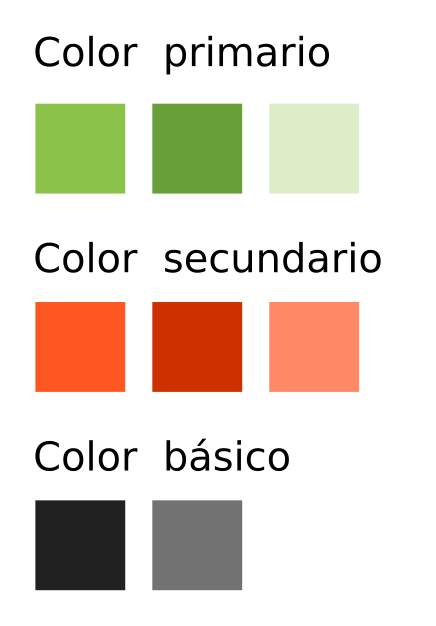
\includegraphics[width=0.3\textwidth]{cap5/img/paleta_colores}
  \caption{Paleta de colores de Amuse Bouche}
  \label{fig:paleta-colores}
\end{figure}


\subsection{Elección de la tipografía}

Siguiendo las directrices del diseño Material, optamos por la fuente Roboto,
por sus características y porque es la fuente por defecto en las nuevas versiones
de Android.

Roboto~\cite{roboto-font} tiene una naturaleza dual. Tiene un esqueleto mecánico y
las formas son en gran parte geométricas. Al mismo tiempo, la fuente cuenta con
curvas suaves y abiertas. Está publicada bajo licencia Apache. La fuente fue
completamente diseñada por el diseñador de interfaces de Google Christian
Robertson, que también diseñó la fuente Titling incluida en el sistema operativo
Ubuntu. 


\section{Diseño de la interfaz de usuario}

En esta sección se detallarán las interfaces visuales de la app del proyecto,
indicando qué acciones realizan cada uno de los componentes que las conforman.

TODO
